\documentclass[tikz,border=4pt]{standalone}
% Shared art direction for the "phones" post, after Vagrancy's region art
% (vagrancy/analysis/art/regions.py and data/palette.json "art"): flat fills,
% plum ink lines, a mustard sky, peach and sage. Every colour below is copied
% from that palette so the post and the game look like one hand drew them.
%
% The scenes share a horizon at y=2.6 and the same sky band, so consecutive
% figures read as one continuous walk down the page.
\usetikzlibrary{arrows.meta,calc,decorations.pathmorphing}
\definecolor{ink}{HTML}{3B2A3F}
\definecolor{sky}{HTML}{E9C46A}
\definecolor{skylight}{HTML}{F2DC98}
\definecolor{cloud}{HTML}{F6E7B8}
\definecolor{peach}{HTML}{EBA77C}
\definecolor{peachdark}{HTML}{D98B5C}
\definecolor{cream}{HTML}{F3E6C4}
\definecolor{sage}{HTML}{9DB58A}
\definecolor{sagedark}{HTML}{6F8F66}
\definecolor{olive}{HTML}{B9B566}
\definecolor{teal}{HTML}{79ADA4}
\definecolor{tealdark}{HTML}{4F8580}
\definecolor{slate}{HTML}{6E8494}
\definecolor{stone}{HTML}{C9B79C}
\definecolor{wood}{HTML}{A9774E}
\definecolor{gold}{HTML}{E3B04B}
\definecolor{shadow}{HTML}{5B4A63}
\tikzset{
  ln/.style={draw=ink, line width=0.9pt, line join=round},
  thinln/.style={draw=ink, line width=0.6pt, line join=round},
  lab/.style={font=\sffamily\scriptsize, text=ink, align=center},
  tag/.style={font=\sffamily\scriptsize\bfseries, text=ink, align=center},
}
% A walking figure. #1 x, #2 y, #3 body colour, #4 head tilt in degrees
% (0 upright, negative looking down at a phone).
\newcommand{\walker}[4]{%
  \begin{scope}[shift={(#1,#2)}]
    \filldraw[fill=#3, ln] (-0.13,0) rectangle (0.13,0.52);
    \draw[ln] (-0.09,0) -- (-0.14,-0.28);
    \draw[ln] (0.09,0) -- (0.17,-0.26);
    \begin{scope}[rotate around={#4:(0,0.52)}]
      \filldraw[fill=cream, ln] (0,0.66) circle (0.14);
    \end{scope}
  \end{scope}}

\begin{document}
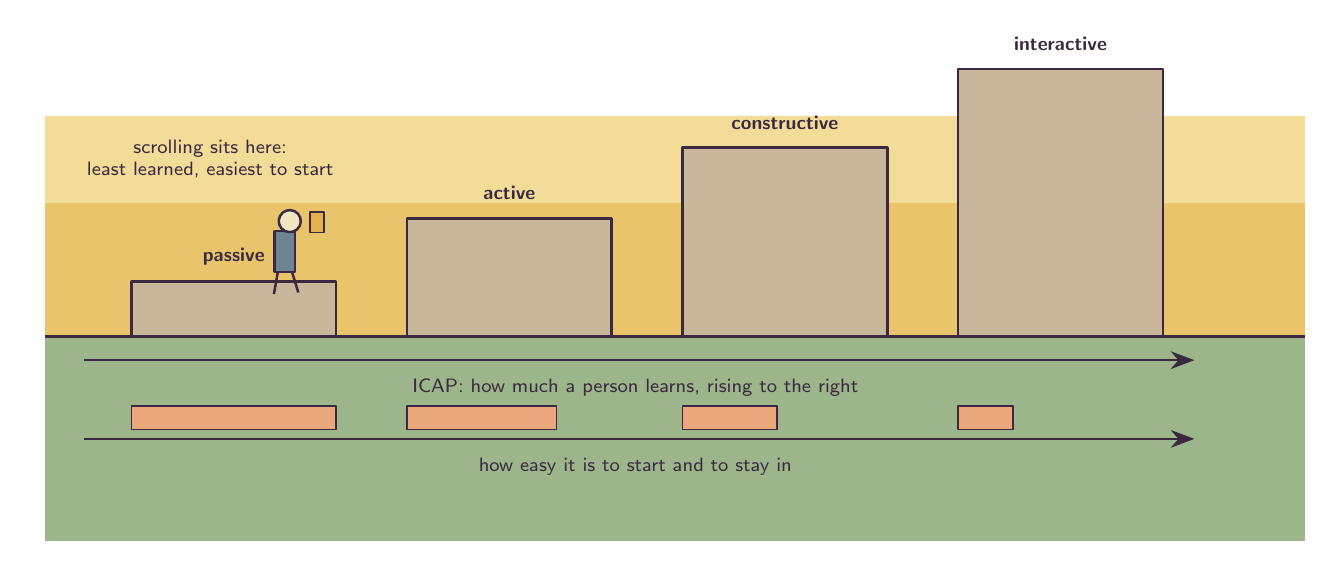
\begin{tikzpicture}[font=\sffamily]
  \fill[sky] (0,2.6) rectangle (16,5.4);
  \fill[skylight] (0,4.3) rectangle (16,5.4);
  \fill[sage] (0,0) rectangle (16,2.6);
  \draw[ln] (0,2.6) -- (16,2.6);
  % ICAP as four rising steps. The height is the learning gain; the walker's
  % effort is drawn separately below, because they are different axes.
  \foreach \i/\x/\h/\name in {0/1.1/0.7/passive, 1/4.6/1.5/active, 2/8.1/2.4/constructive, 3/11.6/3.4/interactive}{
    \filldraw[fill=stone, ln] (\x,2.6) rectangle (\x+2.6,2.6+\h);
    \node[tag] at (\x+1.3,2.6+\h+0.32) {\name};
  }
  \draw[ln, -{Stealth[length=3mm]}] (0.5,2.3) -- (14.6,2.3);
  \node[lab] at (7.5,1.95) {ICAP: how much a person learns, rising to the right};
  % The second axis, which ICAP does not describe.
  \draw[ln, -{Stealth[length=3mm]}] (0.5,1.3) -- (14.6,1.3);
  \node[lab] at (7.5,0.95) {how easy it is to start and to stay in};
  \foreach \x/\w in {1.1/2.6, 4.6/1.9, 8.1/1.2, 11.6/0.7}{
    \filldraw[fill=peach, thinln] (\x,1.42) rectangle (\x+\w,1.72);
  }
  % The walker, on the easiest step.
  \walker{3.05}{3.42}{slate}{-26}
  \filldraw[fill=gold, thinln] (3.37,3.92) rectangle (3.55,4.18);
  \node[lab, text width=4.4cm] at (2.1,4.85) {scrolling sits here:\\least learned, easiest to start};
\end{tikzpicture}
\end{document}
